%
%%% TERMINAL
%
\subsection{Terminal について}
\begin{frame}[containsverbatim]
\frametitle{プログラム開発の流れ}
  \begin{center}
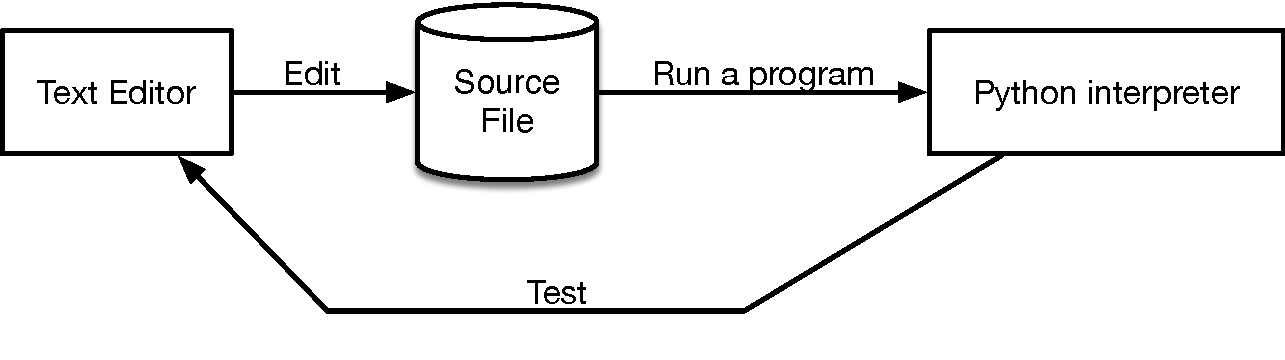
\includegraphics[scale=0.3]{./Figure/CS-figEditAndRun.pdf}
  \end{center}
  \begin{enumerate}
\item テキストエディタを使ってソースファイルを作成
\item ソースファイルを Python インタプリタの上で実行
\item 実行結果が意図したものであるかどうかテスト
  \end{enumerate}
\end{frame}
\begin{frame}[fragile]
\frametitle{ターミナルを使ってみよう}
  \begin{itemize}
\item ターミナルを使ってプログラムを実行してみよう
\item Terminal を起動
\item コマンドプロンプト \verb|>| が表示されたらホームディレクトリの下に適当なディレクトリ (例えば CS1) を作成
\item 作成したディレクトリに cd コマンドで移動してプログラムを実行
  \end{itemize}
  \begin{itembox}{準備}
\scriptsize
    \begin{verbatim}
> mkdir CS1           # 課題用のディレクトリを作成
> cd CS1              # 課題用ディレクトリに移動
> python3 confirm.py  # プログラムを実行
    \end{verbatim}
  \end{itembox}
\end{frame}
%
%%% EDIT SROURCE FILE
%
\subsection{ソースファイルの編集}
\begin{frame}[containsverbatim]
\frametitle{ソースファイルの編集}
  \begin{itemize}
\item テキストエディタと呼ばれるソフトウェアを使って編集
    \begin{itemize}
\item vim, emacs, idle など
    \end{itemize}
\item \href{https://sites.google.com/presystems.xyz/elementarycs/top}{\beamerbutton{https://sites.google.com/presystems.xyz/elementarycs/top}} から動作確認用コードをコピー
\item ターミナルからコマンド入力してエディタを起動
\item 起動したらペイスト
\item 先ほど作成したディレクトリの下にファイルを保存
  \end{itemize}
  \begin{itembox}{editor の起動}
\scriptsize
    \begin{verbatim}
> open -a Emacs
あるいは
> open -a Macvim
あるいは
> open -a Idle
    \end{verbatim}
  \end{itembox}
\end{frame}
%
%%% Run a Program
%
%\subsection{プログラムを走らせてみる}
%\begin{frame}[containsverbatim]
%\frametitle{プログラムを走らせてみる}
%  \begin{itemize}
%\item コマンドプロンプト \verb|>| が表示されたら phtyon3 とソースファイル名と入力して return 
%\item Python プログラムが実行されます
%  \end{itemize}
%  \begin{columns}
%    \begin{column}{0.5\textwidth}
%      \begin{itembox}{\footnotesize Python の起動}
%\scriptsize
%        \begin{verbatim}
%> python3 sub.py
%        \end{verbatim}
%      \end{itembox}
%    \end{column}
%    \begin{column}{0.5\textwidth}
%      \begin{itembox}{\footnotesize Ruby の起動と終了}
%\scriptsize
%        \begin{verbatim}
%> irb
%>> load smile.rb
%>> quit
%        \end{verbatim}
%      \end{itembox}
%    \end{column}
%  \end{columns}
%\end{frame}
